\section{Architektura systemu oraz oprogramowanie podstawowe}

Budowany system wspomagania zarządzania firmą informatyczną skłąda sie
z wielu modułów. Ponieważ niniejszy dokument stanowi dokumentację
projektową jedynie do jednego z modułów na rysunku \ref{fig:labelArchOgol}
zaprezentowano ogólny diagram komponentów na które podzielony jest system.

\begin{figure}[h]
	\centering
	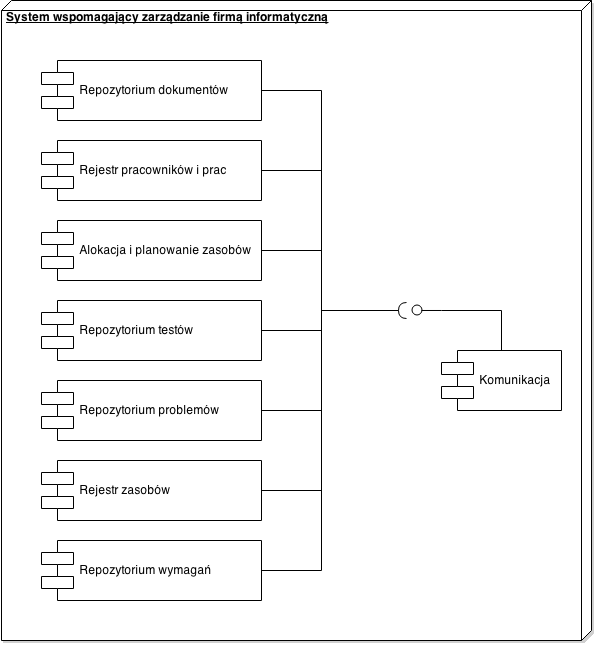
\includegraphics[width=\textwidth]{img/archogol}
	\caption{Diagram komponentów całego systemu\label{fig:labelArchOgol}}
\end{figure}

Bardzo istotnym komponentem systemu jest komponent
komunikacyjny. Został on opisany w osobnym dokumencie wraz ze
szczególami jego interfejsu. Wszystkie pozostałe moduły nie
dostarczają własnych interfejsów lecz korzystają z generycznego
interfejsu dostarczanego przez wspomniany moduł.

Przechodząc zatem do perspektywy omawianego modułu rejestru dostępnych
zasobów system zostanie zrealizowany w architekturze trójwarstwowej z
wykorzystaniem modelu klient-serwer. System będzie składał się z
następujących warstw:

\begin{itemize}
	\item[--] warstwa prezentacji (interfejs użytkownika),
	\item[--] warstwa logiki biznesowej (pośrednicząca w dostępie do danych zapisanych w bazie danych),
	\item[--] warstwa danych.
\end{itemize}

\begin{figure}[h]
	\centering
	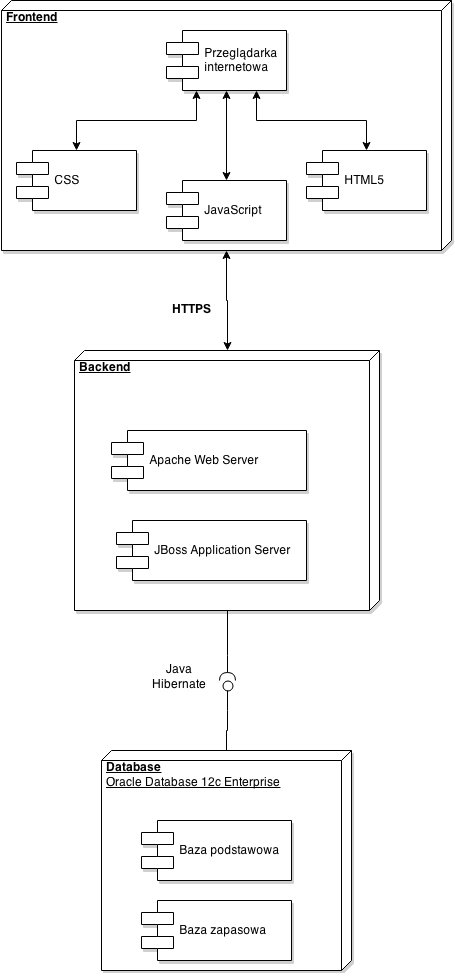
\includegraphics[width=0.8\textwidth]{img/components}
	\caption{Diagram komponentów \label{fig:labelComponents}}
\end{figure}


\subsection{Warstwa prezentacji}

Warstwa prezentacji będzie elementem odpowiedzialnym za prezentację
treści użytkownikowi końcowemu. Będzie również umożliwiać odbieranie
żądań użytkowników i przesyłanie ich do kolejnych warstw. Warstwa ta
zostanie zrealizowana w technologii cienkiego klienta. Dzięki
obecności warstwy prezentacji użytkownicy naszego systemu nie są
zobowiązani do przeprowadzania instalacji dodatkowego oprogramowania w
celu korzystania z jego możliwości - jedynym wymogiem jest posiadanie
przeglądarki internetowej, za pomocą której użytkownik będzie logował
się do systemu. Aby umożliwić prezentację treści użytkownikowi w
przejrzysty sposób przeglądarka po stronie klienta pozwinna obsługiwać
szablony CSS, technologię HTML5 oraz język JavaScript.

\subsection{Warstwa logiki biznesowej}

Warstwa logiki biznesowej będzie składać się ze zbioru komponentów
odpowiedzialnych za spełnianie poszczególnych założeń funkcjonalnych
systemu (o których mowa w niniejszym dokumencie). Zostanie ona
zaimplementowana przy użyciu technologii JavaEE, a jako serwer
aplikacyjny zostanie wykorzystany JBoss Application Server. Do
komunikacji z baza danych wykorzystany zostanie interfejs Java
Hibernate. Całość zostanie zintegrowana z Apache Web Server.

Warstwa aplikacji stanowi najważniejszy element całego systemu i jest
odpowiedzialna za całą logikę zawartą w aplikacji. W związku z
powyższym jest ona dość skomplikowana i składa się z wielu elementów.

\subsection{Warstwa danych}

Warstwa danych odpowiedzialna będzie za dostęp do bazy danych -
odczytywanie i zapisywanie w niej informacji. Do realizacji projektu
wybrano relacyjną bazę danych SQL. Jako system zarządzania bazą danych
zostanie wykorzystany będzie Oracle Database 12c w wersji
Enterprise. W celu zapewnienia trwałości przechowywanych danych oraz
wysokiej dostępności systemu w warstwie tej funkcjonowały będą dwie
instancje bazy danych - podstawowa i zapasowa.

